\chapter{サーバーゾーンでのクラスタ構築における仮想環境を使用した事前検証}
\label{chap:fourth}

\section{緒言}
本章では、サーバーゾーンでのクラスタ構築における仮想環境を使用した事前検証ついて述べる。

\section{サーバーゾーンで稼働しているElasticsearchシステムの状況}
サーバーゾーンでは, 133.71.201.197で単一ノードのElasticsearchが稼働しており, リサイクル館の太陽光パネルの計測データが保存されている.

133.71.201.197のElasticsearchのバージョン7.17.6であり, 学内ゾーンで稼働しているElasticsearchクラスタに参加しているElastisearchノードのバージョンは7.17.9である.

本研究室では現在, バージョン7.17.9のElasticsearchを採用しているため, サーバーゾーンで構築しようとしているクラスタのElasticsearchのバージョンも, 学内ゾーンで稼働しているElasticsearchクラスタと同様, バージョン7.17.9を採用する.

そこで, Docker, Docker Compose を使用して, 異なるバージョンである7.17.6 と 7.17.9 の Elasticsearch ノードをクラスタリングすることが可能かどうかを確認するために実施した.

\section{Dockerとは}
Dockerは, 軽量で独立したコンテナ型仮想環境用のプラットフォームである.

従来の仮想化では, VMWareなどの仮想化ソフトウェアを用いて, ホストOS上にゲストOSを構築する形式だった.
しかし, DockerはホストOS上にゲストOSなしで独立したコンテナ型の仮想環境として構築される.
Dockerコンテナを利用する場合は, Docker Engineをインストールすることでコンテナの立ち上げ, 停止, 削除といった操作を行うことができる.

\begin{figure}
  \begin{center}
    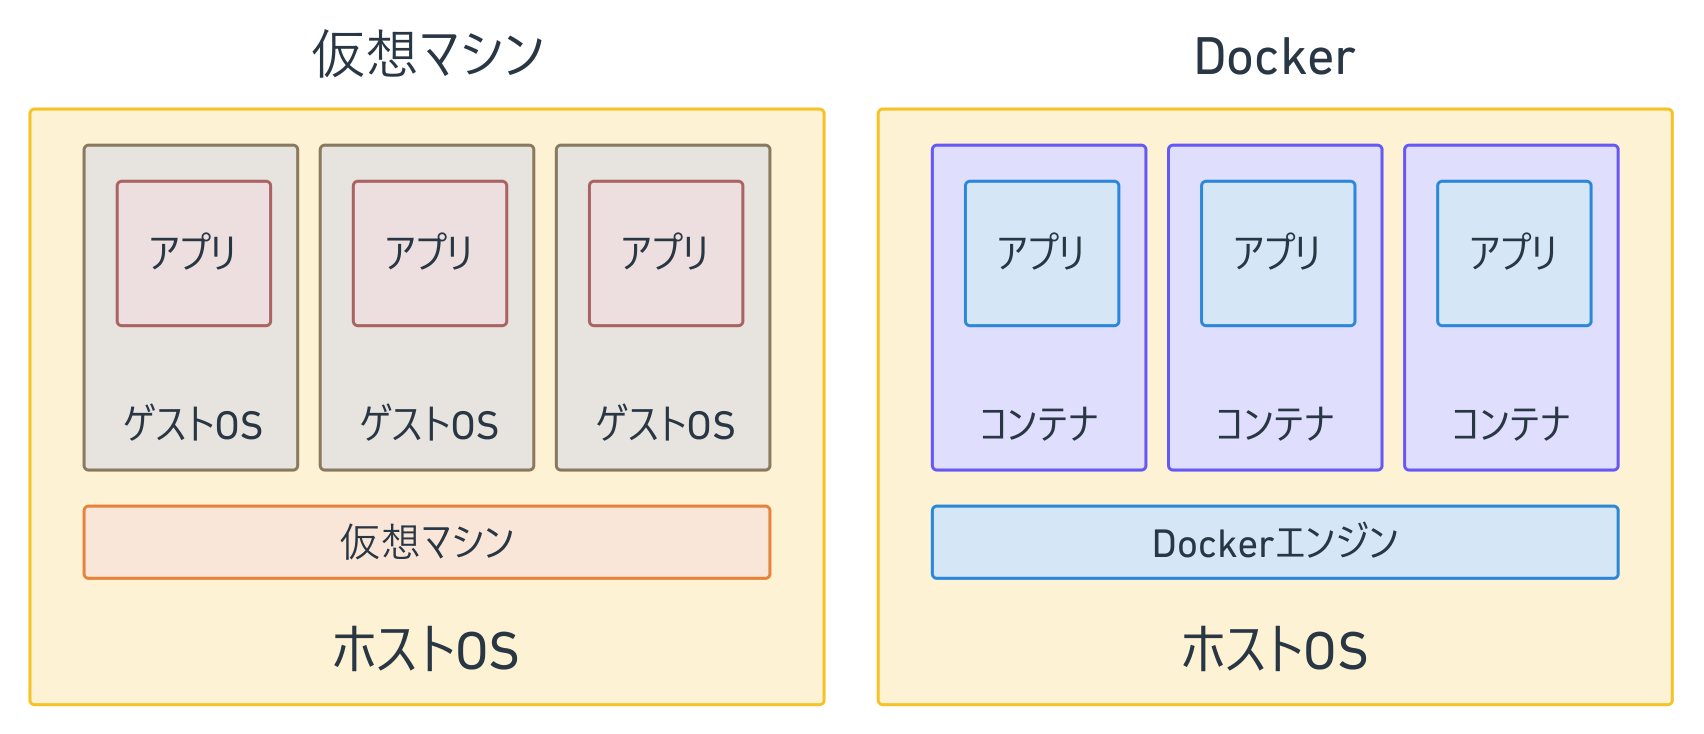
\includegraphics[width=160mm]{sotu/figure/docker-vmware.png}
    \caption{仮想マシンとDockerの違い \cite{2}}
    \label{p0}
  \end{center}
\end{figure}

\subsection{コンテナとは}

コンテナは, アプリケーションとそのすべての依存関係(ライブラリ, 実行環境など)をカプセル化した軽量な実行単位である.
Dockerの場合, コンテナの作成にはDockerイメージが必要となる.

\subsection{Dockerイメージとは}

Dockerイメージとは, Dockerコンテナを作成するためのテンプレートであり, Dockerイメージの中には, Docker コンテナの実行に必要な Linux ファイルシステムとメタ情報を含む.

Linux ファイルシステムというのは,  / ディレクトリ以下の /etc /bin /sbin /usr などのディレクトリ階層およびファイルである. 

Docker では, コンテナとして動かしたいアプリケーションが必要とする, 最小限のファイルを Docker イメージの中に入れる. 

さらに, そのアプリケーションを動かすために必要なデフォルトのコマンドや引数の指定, 外に公開するポート番号の情報などの情報がある. これらをメタ情報として, 同じく Docker イメージの中に入れられる 

DockerイメージはDocker Hubやその他のレジストリで共有されており, これらのサービスから取得することが可能である.

今回はElasticsearchの開発元であるElastic社が提供しているElasticsearchのDockerイメージを使って検証を行う.

\begin{figure}
  \begin{center}
    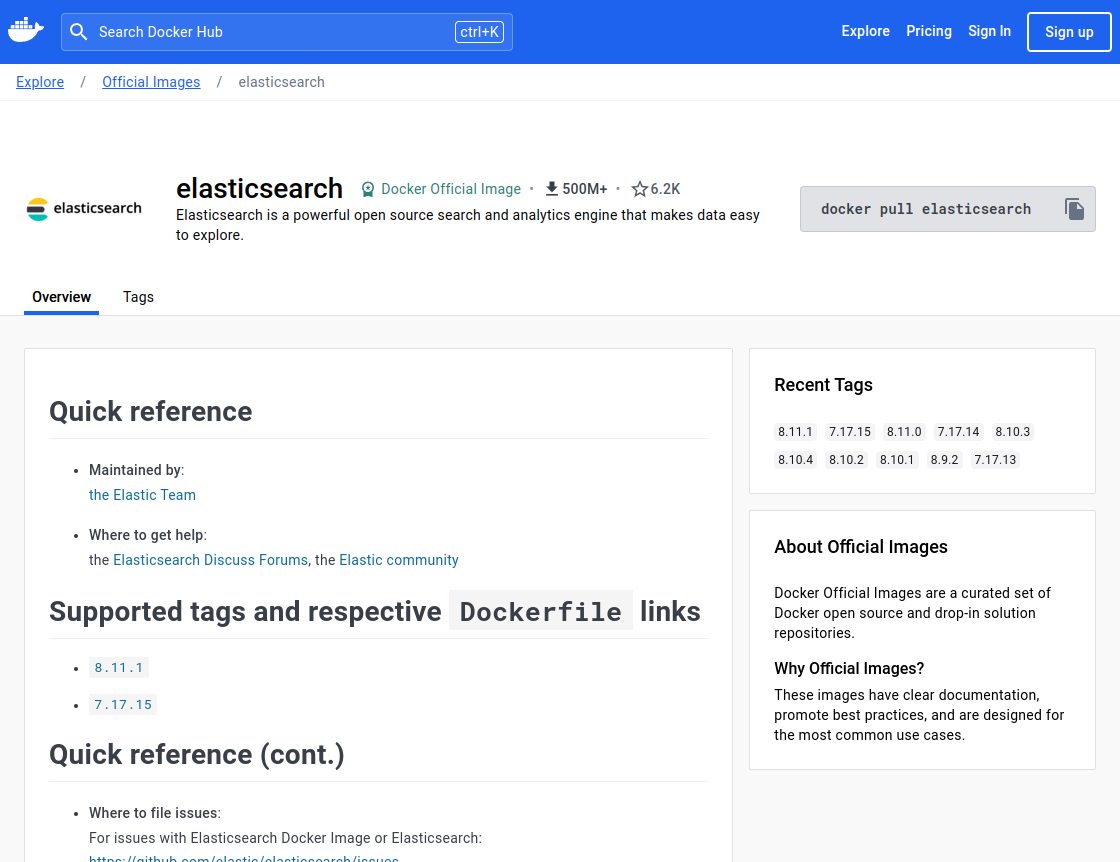
\includegraphics[width=160mm]{sotu/figure/elasticsearch-image.png}
    \caption{ElasticsearchのDockerイメージ}
    \label{s0}
  \end{center}
\end{figure}

\section{Docker Composeとは}
Docker Composeは, 複数のコンテナを定義し, 実行するためのツールである. これはYAMLファイルを使用して設定され, 複数のコンテナで協調して動作するアプリケーションの開発を単純化する.

\section{検証環境のセットアップ}
\subsection{全て同じバージョンのElasticsearchを使用したクラスタ構成 (全ノード バージョン 7.17.9)}

Listing \ref{sc1}に7.17.9バージョンのElasticsearchのみを使用してクラスタを構築した時のdocker-compose.ymlをを示す.

\begin{lstlisting}[caption=全て同じバージョンのElasticsearchを使用したクラスタを構成するdocker-compose.yml, label=sc1]
  version: '2.2'
  services:
    es01:
      image: docker.elastic.co/elasticsearch/elasticsearch:7.17.9
      container_name: es01
      environment:
        - node.name=es01
        - cluster.name=es-docker-cluster
        - discovery.seed_hosts=es02,es03
        - cluster.initial_master_nodes=es01,es02,es03
      ports:
        - 9200:9200
      networks:
        - elastic
    es02:
      image: docker.elastic.co/elasticsearch/elasticsearch:7.17.9
      container_name: es02
      environment:
        - node.name=es02
        - cluster.name=es-docker-cluster
        - discovery.seed_hosts=es01,es03
        - cluster.initial_master_nodes=es01,es02,es03
      networks:
        - elastic
    es03:
      image: docker.elastic.co/elasticsearch/elasticsearch:7.17.9
      container_name: es03
      environment:
        - node.name=es03
        - cluster.name=es-docker-cluster
        - discovery.seed_hosts=es01,es02
        - cluster.initial_master_nodes=es01,es02,es03
      networks:
        - elastic
  
  networks:
    elastic:
      driver: bridge
  \end{lstlisting}

また, 図 \ref{d1}にListing \ref{sc1}のdocker-compose.ymlを図で表現したものを示す.

\begin{figure}
  \begin{center}
    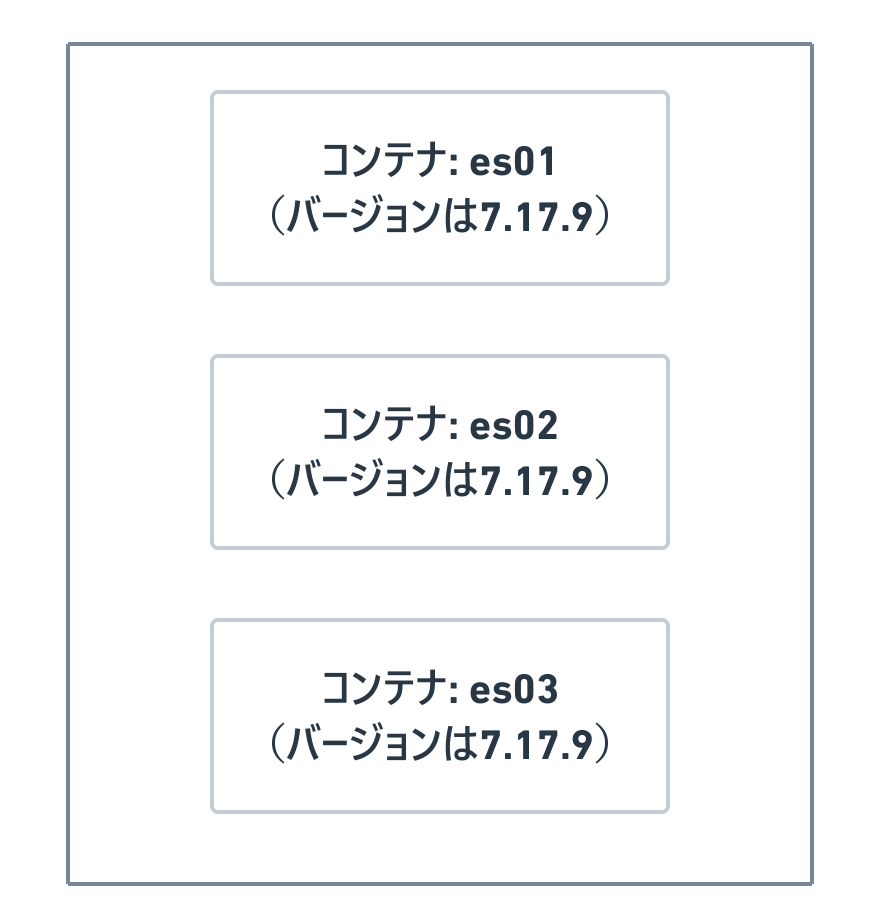
\includegraphics[width=160mm]{sotu/figure/all-7.19.9.png}
    \caption{docker-compose.ymlを図で表現したもの}
    \label{d1}
  \end{center}
\end{figure}

Listing \ref{sc1}のdocker-compose.ymlファイルで記述している内容について説明する.

\subsubsection*{サービスの定義}
\begin{itemize}
  \item \textbf{es01, es02, es03}: これらはElasticsearchのノード(サーバー)である. 各ノードは異なるコンテナとして定義されている. es01, es02, es03はそれぞれ異なるコンテナ名で, Elasticsearchの異なるインスタンスを実行する.
\end{itemize}

\subsubsection*{各ノードの設定}
\begin{itemize}
  \item \textbf{image}: 使用するDockerイメージ. ここではElasticsearchの7.17.9バージョンを使用している.
  \item \textbf{container\_name}: コンテナに割り当てられる名前.
  \item \textbf{environment}: 環境変数の設定. Elasticsearchのクラスタ設定を含む.
  \item \textbf{ports}: ホストマシンとコンテナ間のポートマッピング. 例えば, `9200:9200`はホストマシンの9200ポートをコンテナの9200ポートにマッピングする.
  \item \textbf{networks}: コンテナ間通信のためのネットワーク設定. ここではelasticネットワークが使用されている.
\end{itemize}

\subsubsection*{ボリュームとネットワークの設定}
\begin{itemize}
  \item \textbf{networks}: デフォルトのドライバであるbridgeドライバを使用するelasticネットワークを定義している. これにより, 異なるコンテナが相互に通信できるようになる.
\end{itemize}

この設定により, Elasticsearchの3ノードを含むクラスタがDocker上で動作するようセットアップされる.

以降, 説明を簡単にするため, docker-compose.ymlを図で表現したもののみを掲示する.

クラスタの起動には, docker compose up -dコマンドを使用する.

docker compose up -dコマンドを実行した後, curlコマンドを使用してクラスタに参加しているノードを一覧表示した結果を図 \ref{p1}に示す.

\begin{figure}
  \begin{center}
    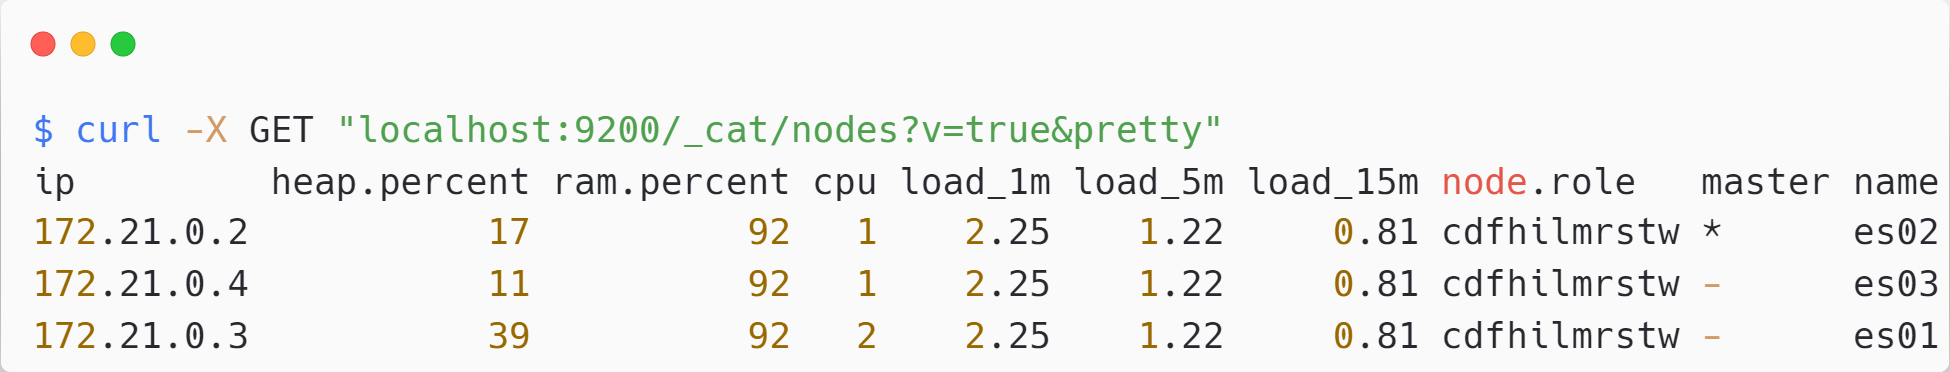
\includegraphics[width=160mm]{sotu/figure/curl-same.png}
    \caption{クラスタに参加しているノードを一覧表示した結果}
    \label{p1}
  \end{center}
\end{figure}

図 \ref{p1}より, 3つのノード(es01, es02, es03)すべてが正常にクラスタに参加できていることが確認できる.

\subsection{異なるバージョンのElasticsearchを使用したクラスタ構成 (2ノード バージョン 7.17.9, 1ノード バージョン 7.17.6)}

図 \ref{d1}のdocker-compose.ymlのes03のコンテナが使用するDockerイメージを変更して, es03のノードで使用するElasticsearchのバージョンを7.17.9から7.17.6に変更する.

図 \ref{d2}に変更後のdocker-compose.ymlを図で表現したものを示す.

\begin{figure}
  \begin{center}
    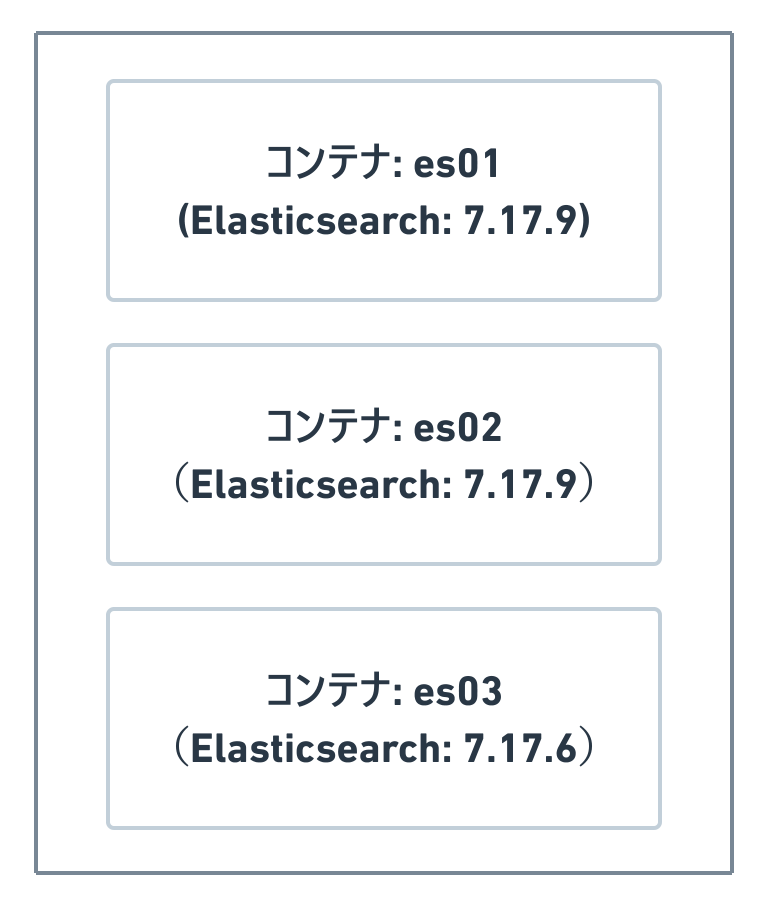
\includegraphics[width=160mm]{sotu/figure/2-7.19.9-and-1-7.17.6.png}
    \caption{変更後のdocker-compose.ymlを図で表現したもの}
    \label{d2}
  \end{center}
\end{figure}

変更後, docker compose up -dコマンドを実行してクラスタを起動する.

クラスタの起動後, curlコマンドを使用してクラスタに参加しているノードを一覧表示した結果を図 \ref{p2}に示す.

\begin{figure}
  \begin{center}
    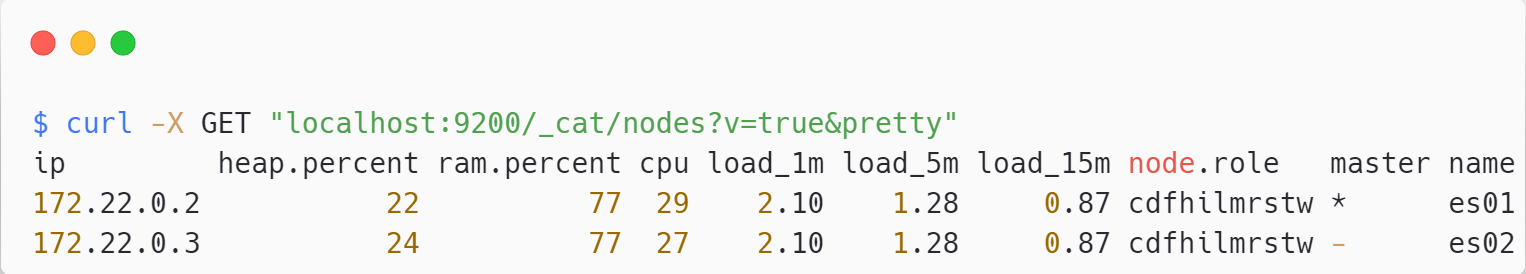
\includegraphics[width=160mm]{sotu/figure/curl-different.png}
    \caption{クラスタに参加しているノードを一覧表示した結果}
    \label{p2}
  \end{center}
\end{figure}

図 \ref{p2}より, バージョンが7.17.9である2つのノード(es01, es02)のみが正常にクラスタに参加できていることが確認できる.

また, Elasticsearch起動時に出力されたログを確認したところ, 図 \ref{p3}に示すように, クラスタに参加できなかったes03のコンテナでElasticsearchがエラーログを出力して終了していることが分かった.

\begin{figure}
  \begin{center}
    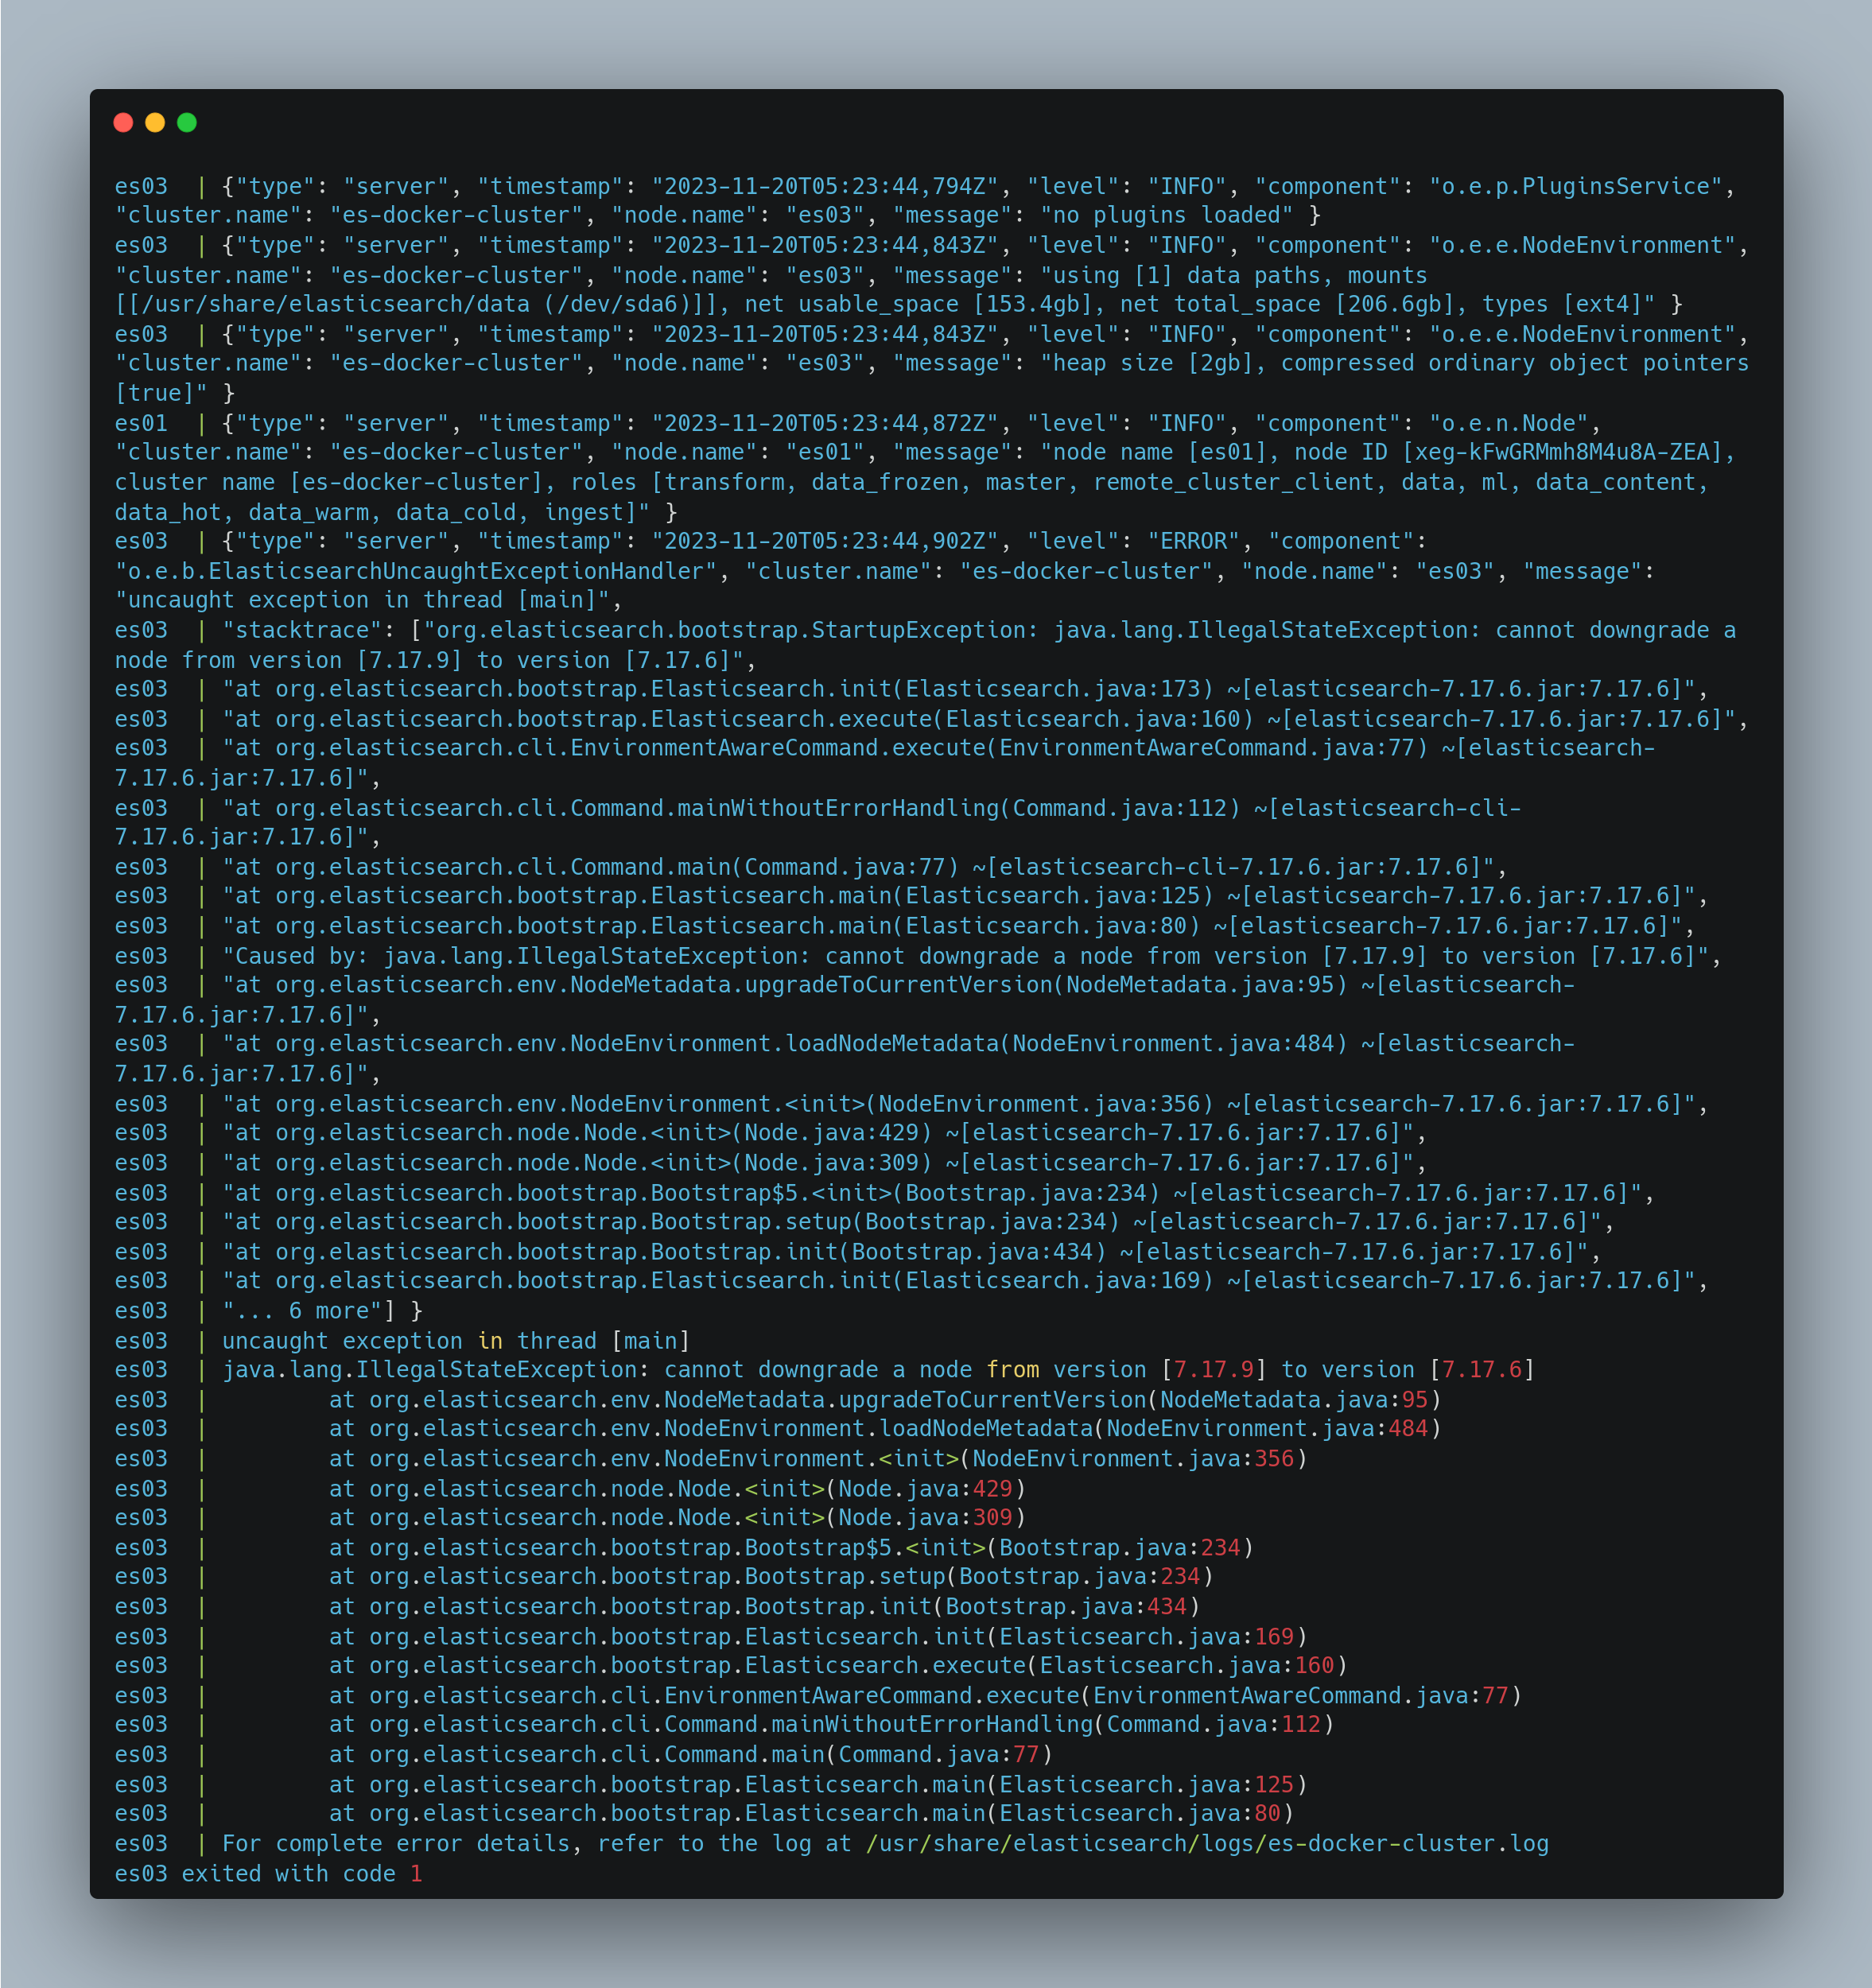
\includegraphics[width=160mm]{sotu/figure/log.png}
    \caption{es03のログ}
    \label{p3}
  \end{center}
\end{figure}

\section{異なるElasticsearchクラスタへのノード参加検証}
サーバーゾーンでのクラスタ構築において, リサイクル館の太陽光パネルの計測データを保存しているElasticsearchノードを新たなノードとして構築したクラスタに参加できるか, Dockerを用いて検証した.

\section{手順}

\subsection{単一ノードで稼働するクラスタAの構築}

まず, docker-composeを用いて単一ノード(コンテナ名はes04)でクラスタ以後このクラスタをクラスタAと呼ぶを構築する. 以後このクラスタをクラスタAと呼ぶ.

図 \ref{d3}にクラスタAの構築の際に使用したdocker-compose.ymlを図で表現したものを示す.

\begin{figure}
  \begin{center}
    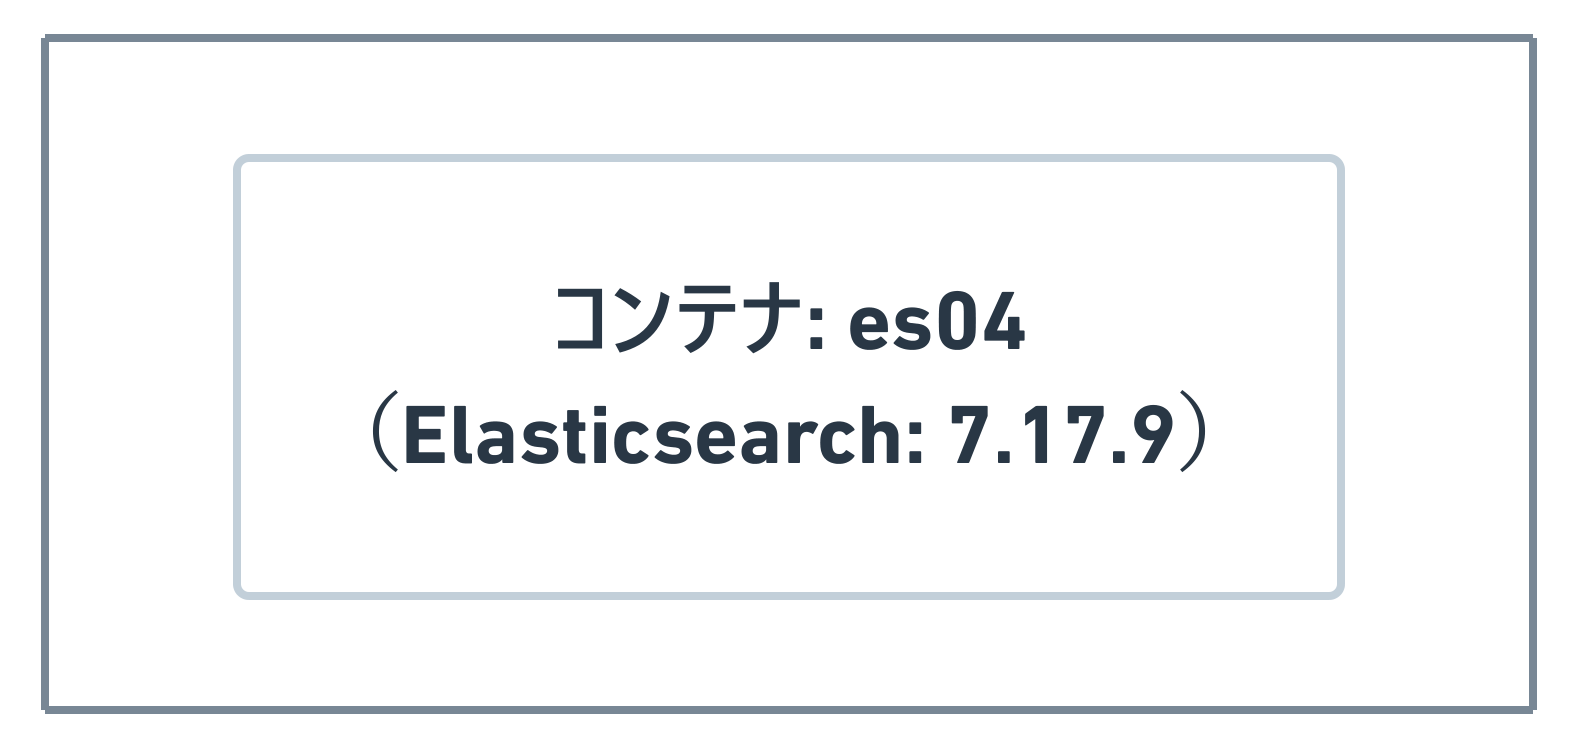
\includegraphics[width=160mm]{sotu/figure/1-7.17.9.png}
    \caption{クラスタAの構築の際に使用したdocker-compose.ymlを図で表現したもの}
    \label{d3}
  \end{center}
\end{figure}

docker-composeを用いてノードを起動した後, クラスタの情報について問い合わせた結果を図 \ref{p1-1}に示す.

\begin{figure}
  \begin{center}
    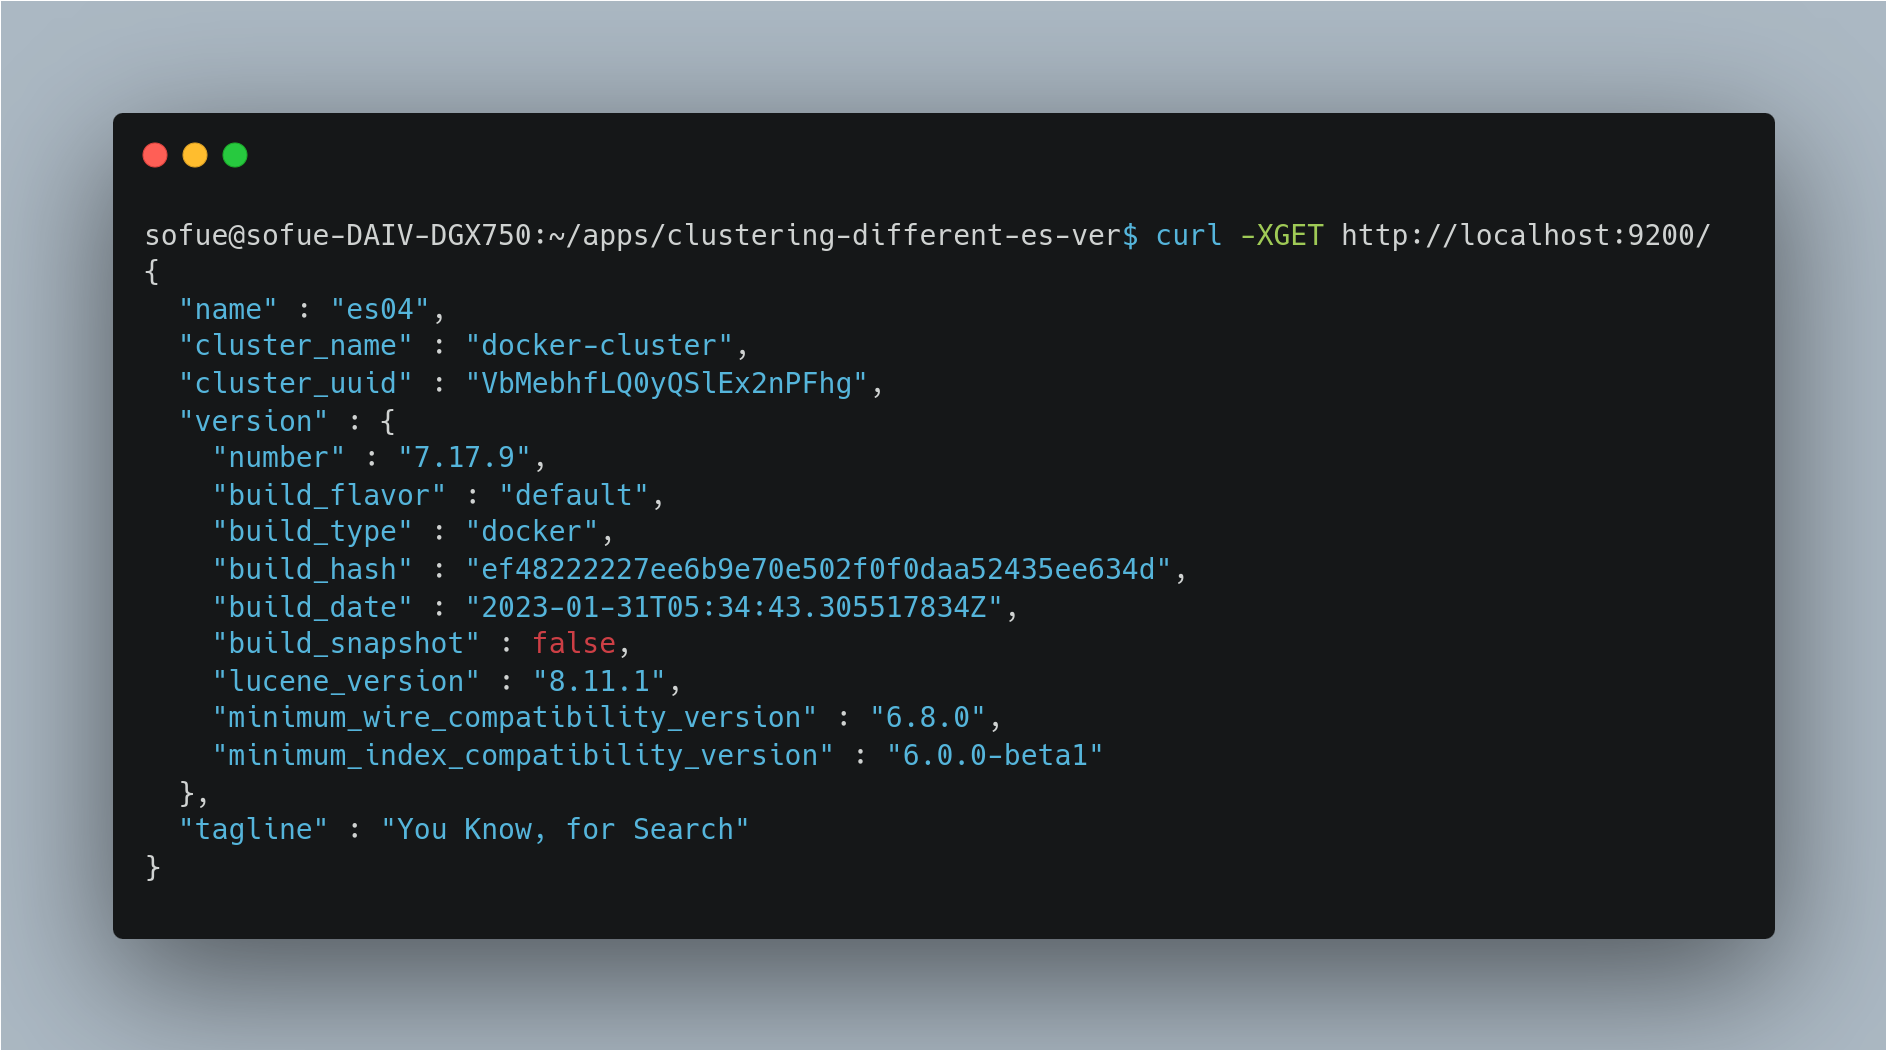
\includegraphics[width=160mm]{sotu/figure/es04-cluster.png}
    \caption{クラスタの情報について問い合わせた結果}
    \label{p1-1}
  \end{center}
\end{figure}

クラスタの情報について問い合わせた後, Dockerコンテナを停止してノードをシャットダウンした.

\subsection{クラスタBの構築}

次に, クラスタAに使用したノードとは別の3ノード(コンテナ名はそれぞれes01, es02, es03)でクラスタを構築する. 以後このクラスタをクラスタBと呼ぶ.

図 \ref{d4}にクラスタBの構築の際に使用したdocker-compose.ymlを図で表現したものを示す.

\begin{figure}
  \begin{center}
    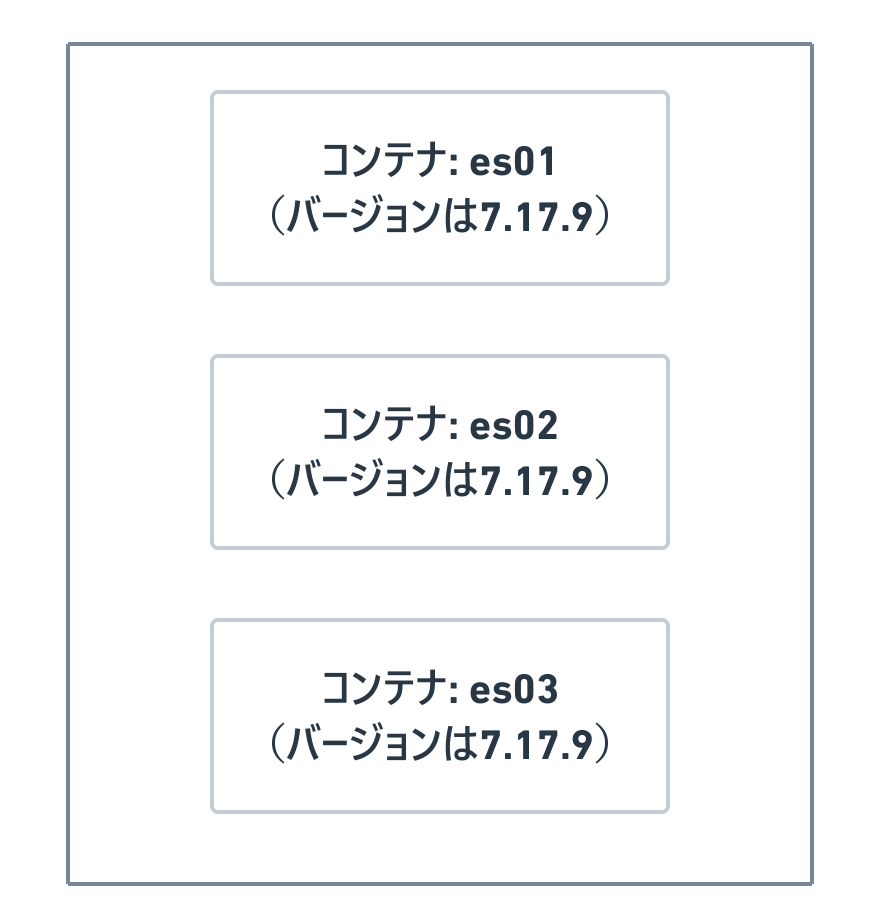
\includegraphics[width=160mm]{sotu/figure/all-7.19.9.png}
    \caption{クラスタBの構築の際に使用したdocker-compose.ymlを図で表現したもの}
    \label{d4}
  \end{center}
\end{figure}

docker-composeを用いて3つのノードを起動した後, クラスタの情報について問い合わせた結果を図 \ref{p2-1}に示す.

\begin{figure}
  \begin{center}
    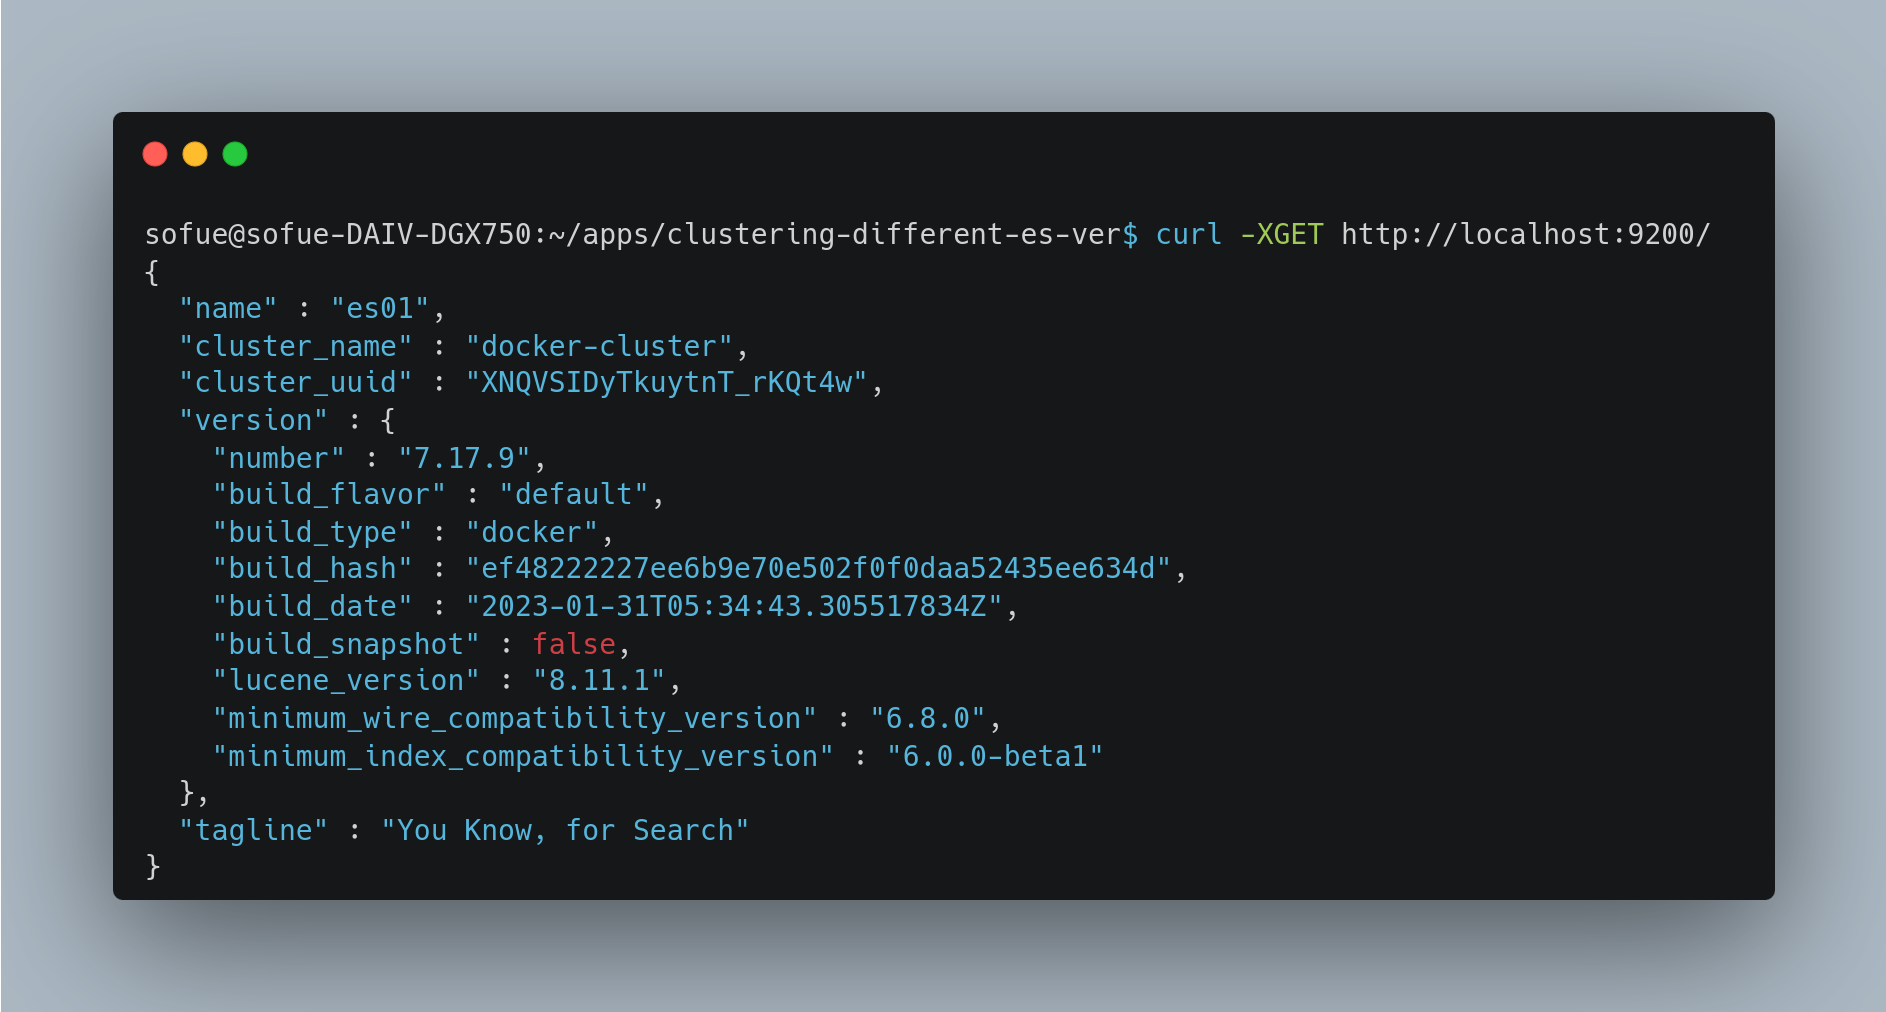
\includegraphics[width=160mm]{sotu/figure/3nodes-cluster.png}
    \caption{クラスタの情報について問い合わせた結果}
    \label{p2-1}
  \end{center}
\end{figure}

図 \ref{p1-1}, \ref{p2-1}より, クラスタAとクラスタBはそれぞれ異なるクラスタIDを付与されたことが分かる.

クラスタの起動後, クラスタに参加しているノードの一覧を取得した結果を図 \ref{p2-2}に示す.

\begin{figure}
  \begin{center}
    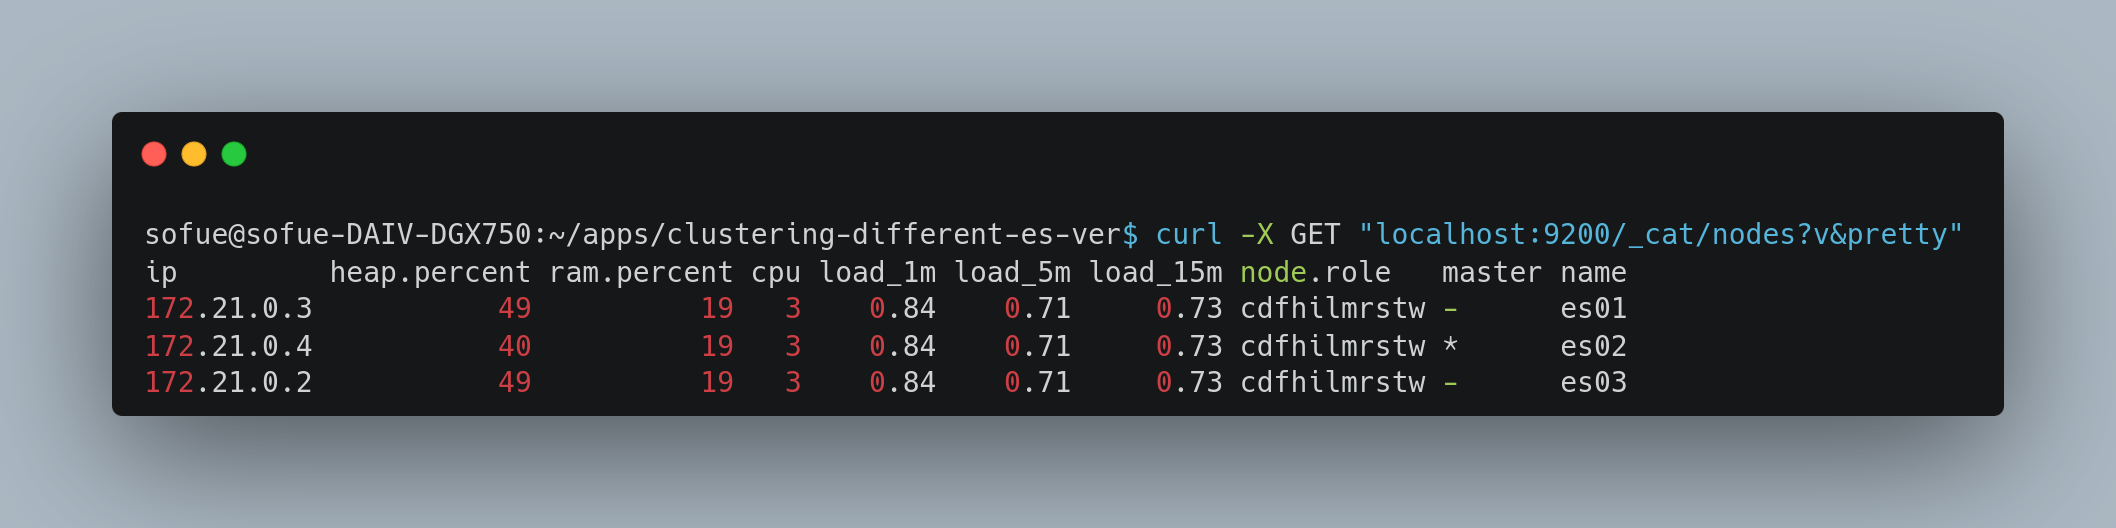
\includegraphics[width=160mm]{sotu/figure/3nodes-list.png}
    \caption{クラスタBの起動後, クラスタに参加しているノードの一覧を取得した結果}
    \label{p2-2}
  \end{center}
\end{figure}

図 \ref{p2-2}より, es01, es02, es03ノードが全てクラスタBに参加できていることが分かる.

クラスタに参加しているノードの一覧を取得した後, 全てのDockerコンテナを停止してノードを全てシャットダウンした.

\subsection{クラスタBへの参加試行}

次に, 図 \ref{d4}のdocker-compose.ymlに対して, クラスタAのノード(es04コンテナ)を追加し, 合計4ノードでのクラスタBの起動を試みる.

図 \ref{d5}に, 合計4ノードでクラスタBの起動を試みた際に使用したdocker-compose.ymlを図で表現したものを示す.

\begin{figure}
  \begin{center}
    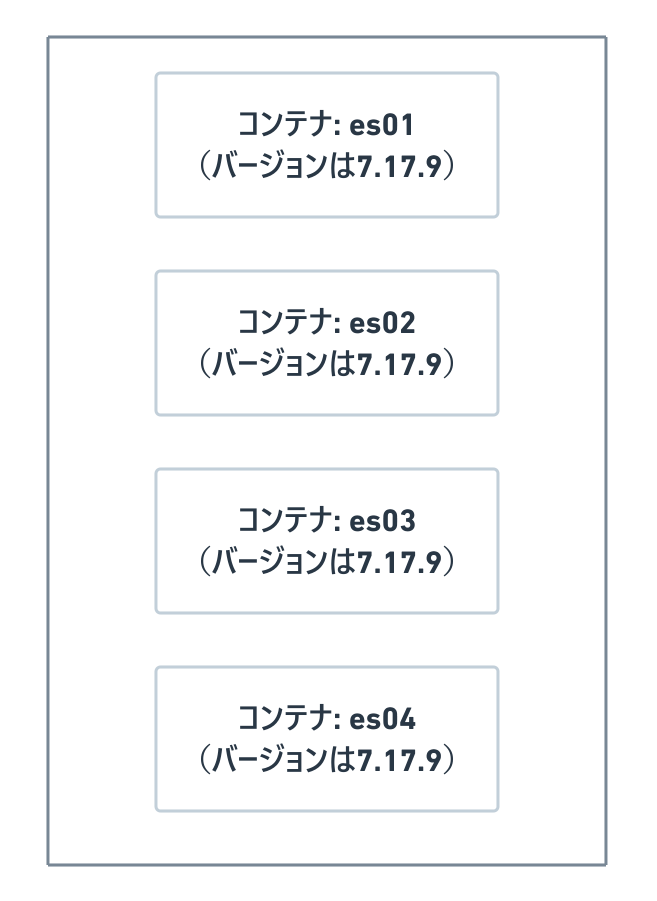
\includegraphics[width=160mm]{sotu/figure/4-7.17.9.png}
    \caption{合計4ノードでクラスタBの起動を試みた際に使用したdocker-compose.ymlを図で表現したもの}
    \label{d5}
  \end{center}
\end{figure}

クラスタの起動後, クラスタに参加しているノードの一覧を取得した結果を図 \ref{p3-1}に示す.

\begin{figure}
  \begin{center}
    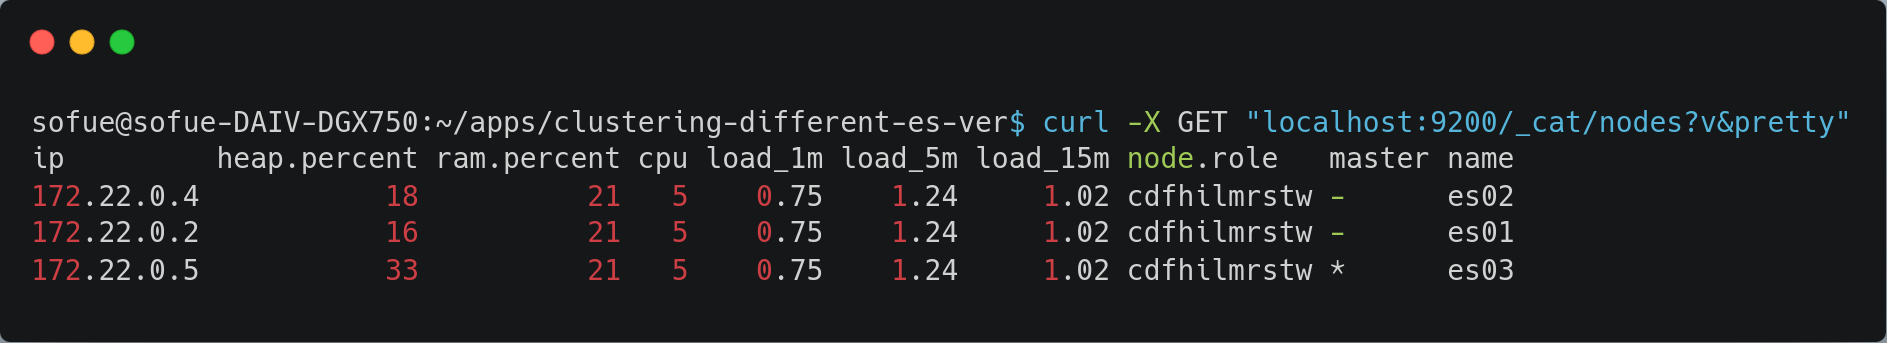
\includegraphics[width=160mm]{sotu/figure/4nodes-list.png}
    \caption{合計4ノードでクラスタの起動を試みた後, クラスタに参加しているノードの一覧を取得した結果}
    \label{p3-1}
  \end{center}
\end{figure}

図 \ref{p3-1}より, クラスタAのノードがクラスタBに参加できていないことが分かる.

es04コンテナ(クラスタAのノード)で出力されたログの一部を図 \ref{p3-2}に示す.

\begin{figure}
  \begin{center}
    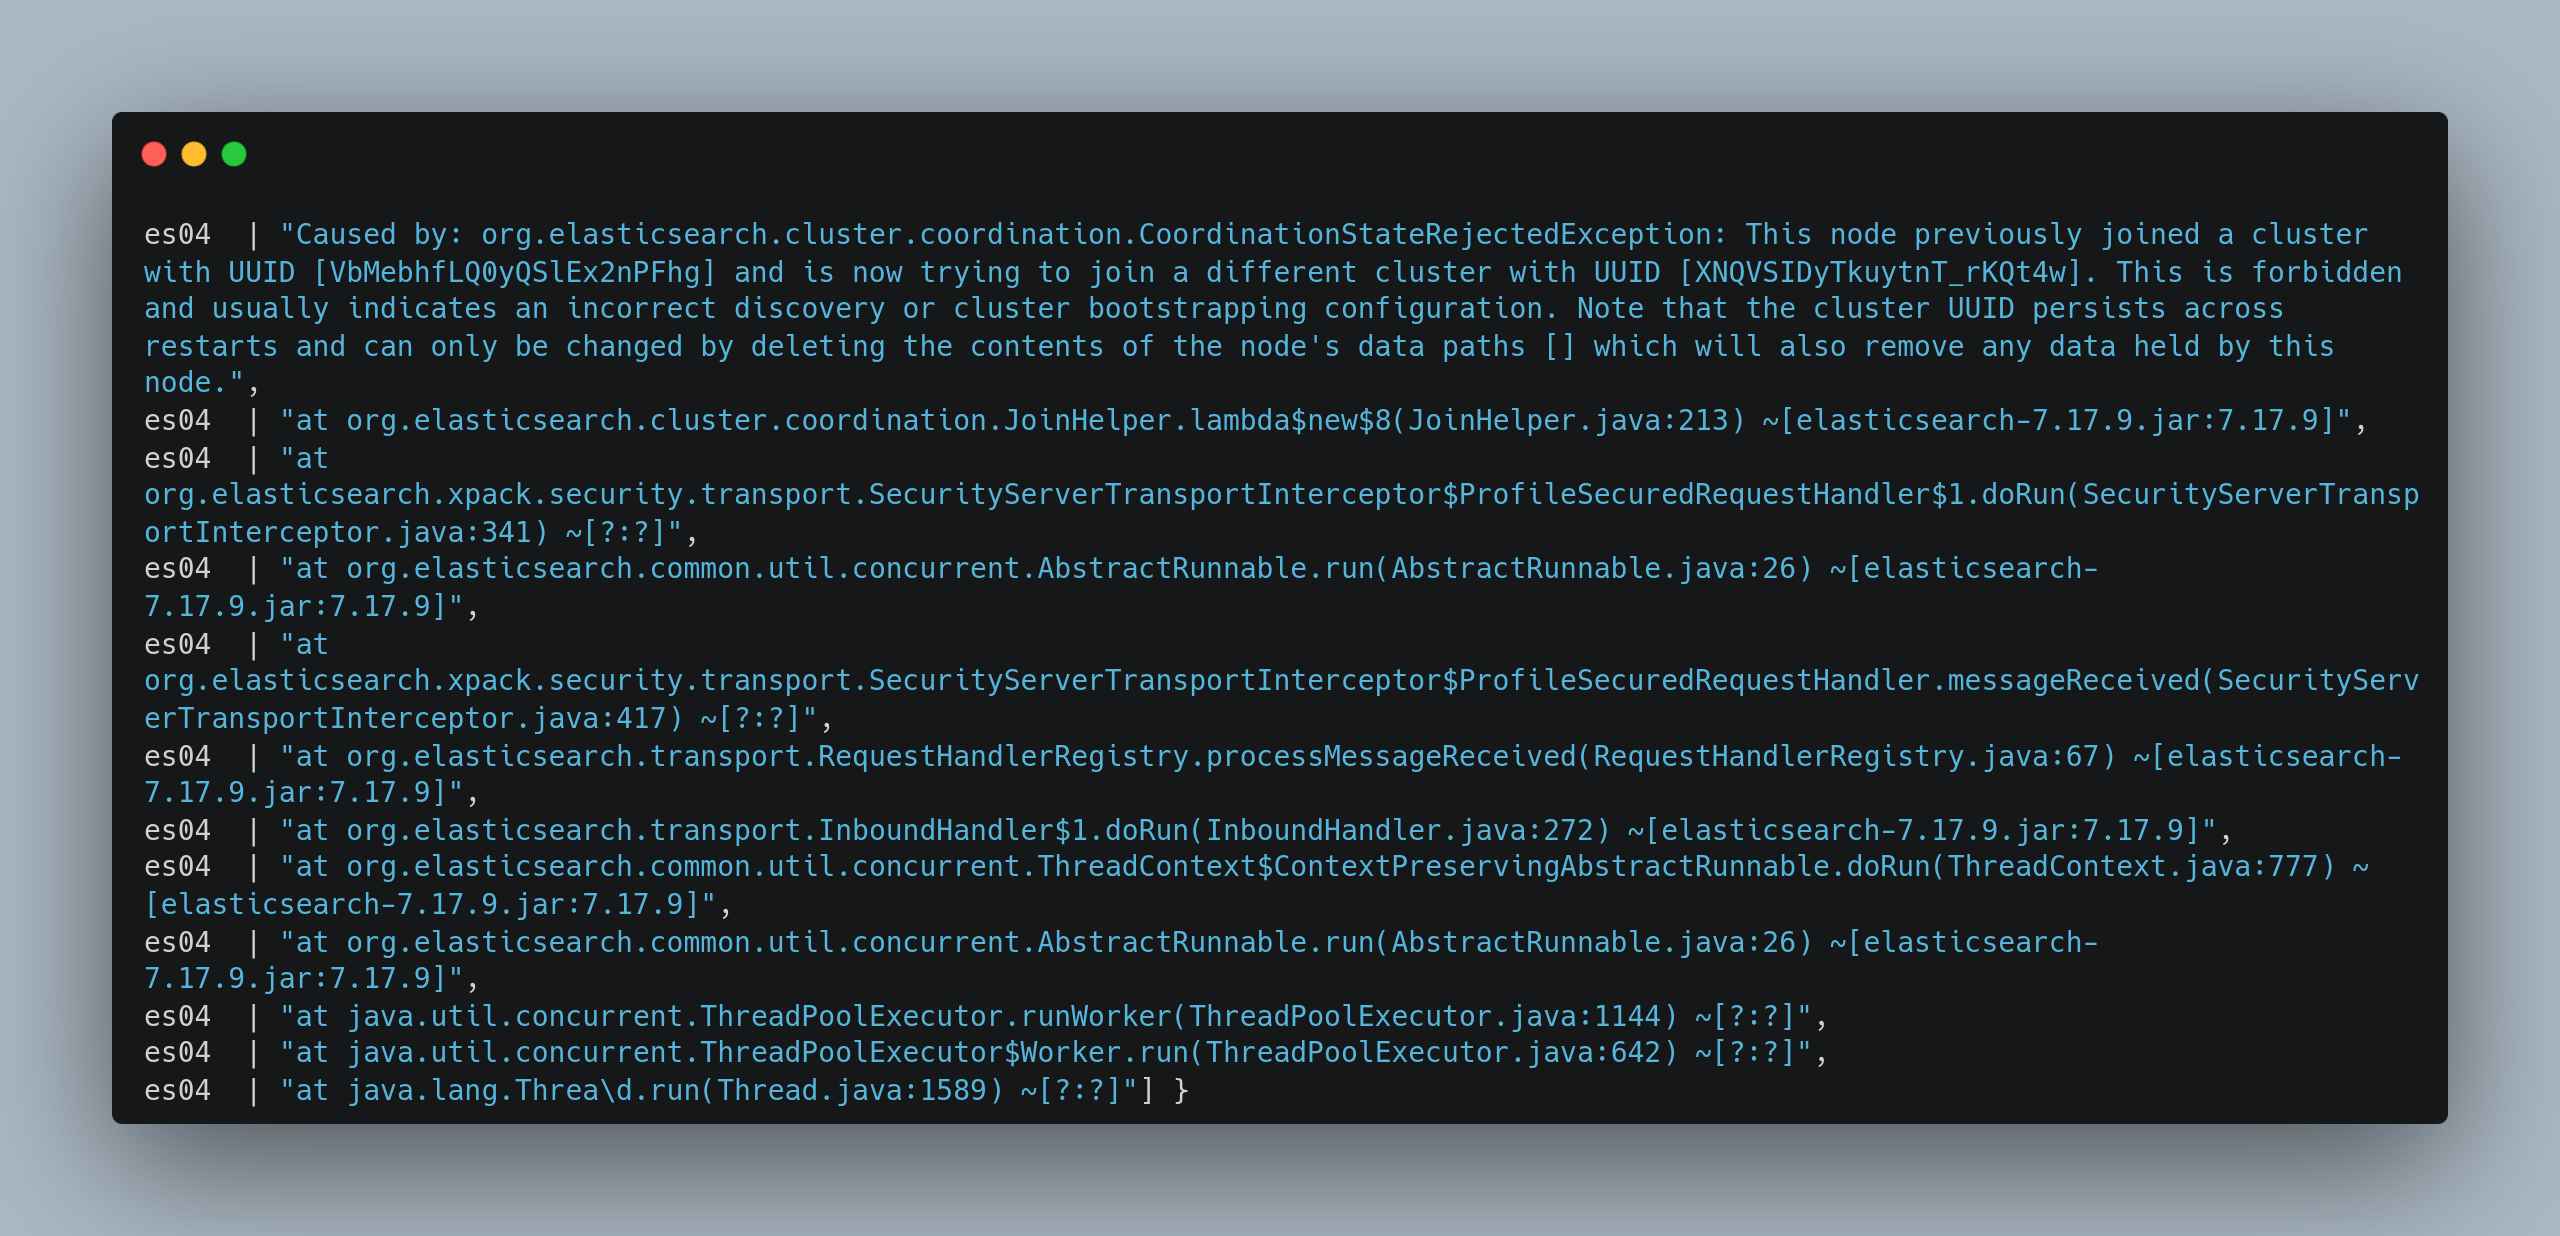
\includegraphics[width=160mm]{sotu/figure/es04-log.png}
    \caption{es04コンテナのログ}
    \label{p3-2}
  \end{center}
\end{figure}

図 \ref{p3-2}には, 異なるクラスタIDを持つクラスタにノードが参加することは禁止されており, これを行うためにはインデックスやドキュメント情報などが格納されているデータパス配下のフォルダ, ファイルを削除する必要があると書かれている.

以上の検証結果から, 既に稼働しているノードを別のクラスタに新しいノードとして参加させることは出来ないことが分かった.

したがって, リサイクル館の太陽光パネルの計測データが保存されたElasticsearchノードをクラスタに参加させるには以下の2通りの方法が考えられる.

\begin{itemize}
  \item リサイクル館の太陽光パネルの計測データが保存されたElasticsearchノードのバックアップを取り, ノードに保存されたインデックスやドキュメントのデータを削除した上で, CO\textsubscript{2}データなどが保存されたクラスタに新しいノードとして参加させる
  \item CO\textsubscript{2}データなどが保存されたクラスタとは別で, サーバーゾーンに新たにクラスタを構築する. クラスタの構築にはリサイクル館の太陽光パネルの計測データが保存されたElasticsearchノードが所属するクラスタを使用する.
\end{itemize}

% 本来であれば、次の章の内容

\section{Elasticsearchのバージョンアップ}
3章の検証結果より, 異なるバージョンのElasticsearchノードでクラスタを構築することは出来ないため, リサイクル館の太陽光パネルの計測データを保存しているElasticsearch(133.71.201.197)をバージョンアップする必要がある. そこで, 133.71.201.197にインストールされたElasticsearchのバージョンアップを行う.

\section{バージョンアップ手順}

\subsection{インストール方法の特定}

バージョンアップを行うためには, 133.71.201.197のUbuntuPCにどのようにElasticsearchをインストールしたか特定する必要がある.

図 \ref{4-p1}に, aptによってインストールされたパッケージの中にelasticsearchという文字列を含むパッケージが存在するか調べた結果を示す.
図 \ref{4-p1}より, aptによってインストールされたことが分かった.

\begin{figure}
  \begin{center}
    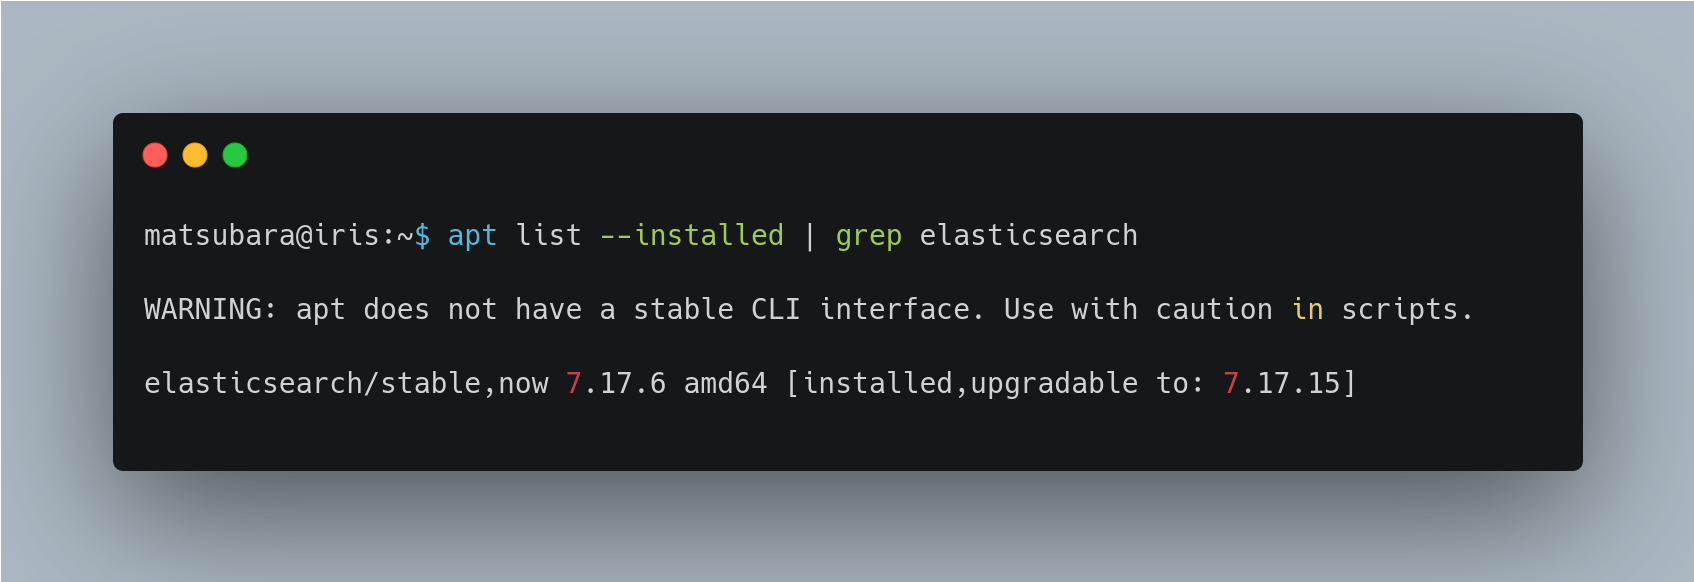
\includegraphics[width=160mm]{sotu/figure/apt-grep.png}
    \caption{aptによってelasticsearchがインストールされたか調べた結果}
    \label{4-p1}
  \end{center}
\end{figure}

次に, aptでインストール可能なelasticsearchのバージョンを一覧表示した結果を図 \ref{4-p2}に示す. 図 \ref{4-p2}にターゲットである7.17.9が含まれているため, aptを使用してバージョンアップできることが確認できた.

\begin{figure}
  \begin{center}
    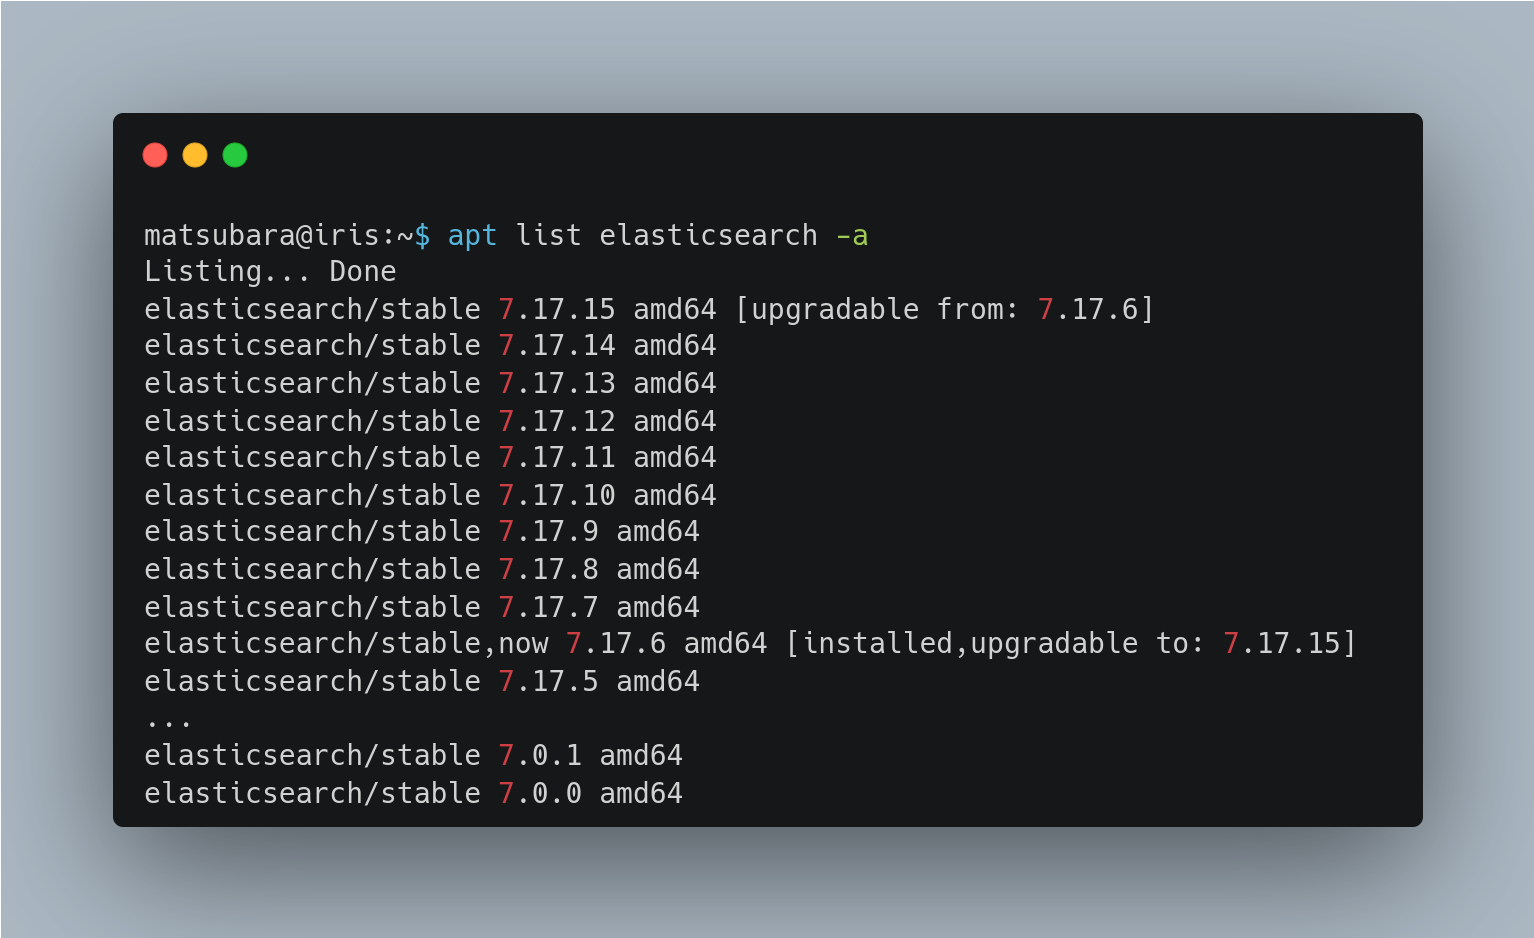
\includegraphics[width=160mm]{sotu/figure/apt-list.png}
    \caption{aptでインストール可能なelasticsearchのバージョンを一覧表示した結果}
    \label{4-p2}
  \end{center}
\end{figure}

\subsection{aptによるバージョンアップ}

まず, \textbf{sudo systemctl stop elasticsearch.service}コマンドを実行してelasticsearchノードをシャットダウンする.

次に, \textbf{sudo apt install elasticsearch=7.17.9}コマンドを実行してelasticsearchパッケージをバージョンアップする.

elasticsearchをバージョンアップ後, \textbf{sudo systemctl start elasticsearch}コマンドを実行してElasticsearchノードを起動する.

ノードの起動後, Elasticsearchのバージョンを確認した結果を図 \ref{4-p3}に示す.

\begin{figure}
  \begin{center}
    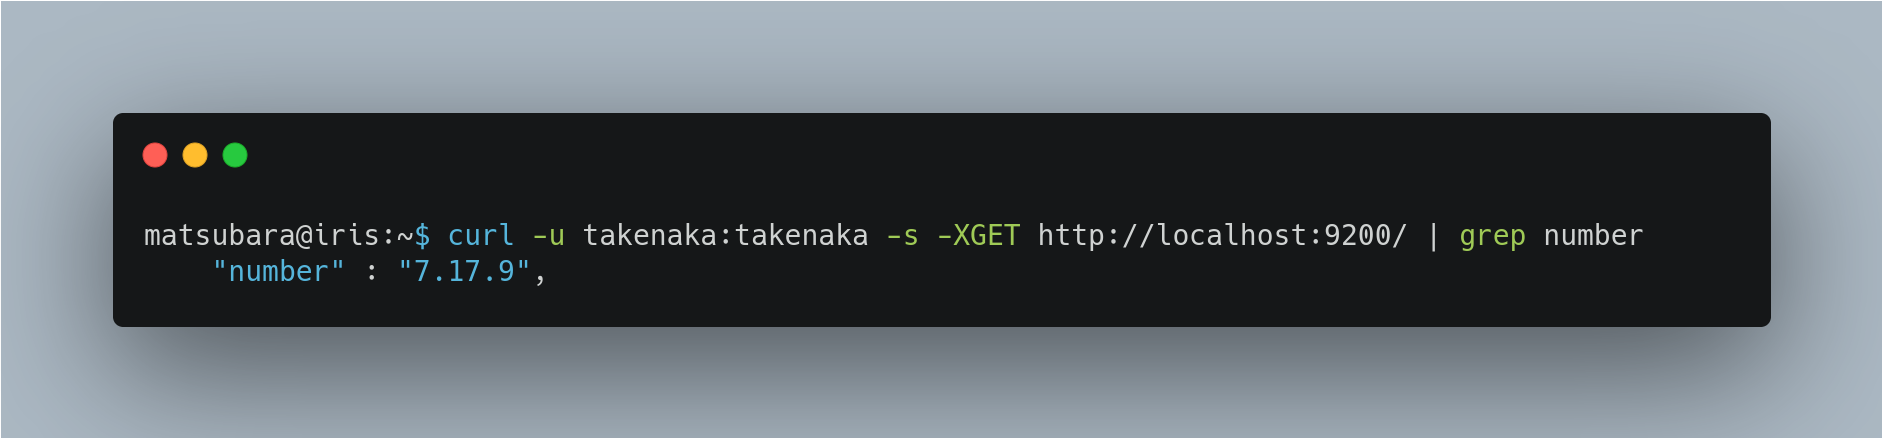
\includegraphics[width=160mm]{sotu/figure/version-check.png}
    \caption{ノードの起動後, Elasticsearchのバージョンを確認した結果}
    \label{4-p3}
  \end{center}
\end{figure}

図 \ref{4-p3}より, Elasticsearchのバージョンが7.17.9にバージョンアップ出来たことが確認できた.

\section{kibanaのバージョンアップ}

kibanaもelasticsearchと同様, aptを使用してインストールされていたため, \textbf{sudo systemctl stop kibana.service}コマンド, \textbf{sudo apt install kibana=7.17.9}コマンド, \textbf{sudo systemctl start kibana}コマンドをそれぞれ実行して, kibanaのバージョンアップも行った.

\section{バージョンアップ後の動作確認}

Elasticsearchのバージョンアップ後, 太陽光パネルの計測データがElasticsearchに保存されているかkibana上で確認した結果を図 \ref{p4}に示す.

\begin{figure}
  \begin{center}
    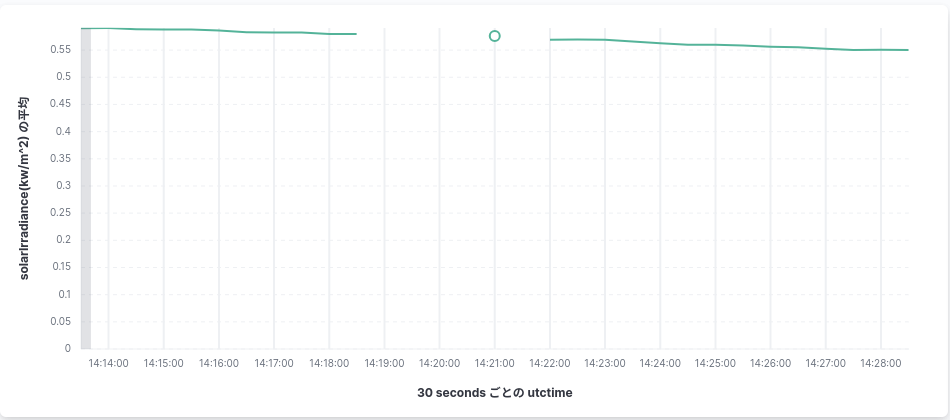
\includegraphics[width=160mm]{sotu/figure/downtime.png}
    \caption{Elasticsearchのバージョンアップ後, 太陽光パネルの計測データが保存されているかkibana上で確認した結果}
    \label{4-p4}
  \end{center}
\end{figure}

図 \ref{4-p4}より, バージョンアップ後のElasicsearchノードを起動した14:22:00以降にドキュメントがインサートされていることが確認できた.

\section{サーバーゾーンにおけるクラスタの構築}

\section{結言}
本章では、サーバーゾーンでのクラスタ構築における仮想環境を使用した事前検証について述べた.

次章ではサーバーゾーンでのクラスタ構築について述べる。
